\documentclass{article}
\usepackage{graphicx}
\usepackage{amsmath}
\usepackage{cite}
\usepackage{geometry}
\geometry{
    letterpaper,
    left=1in,
    right=1in,
    top=1in,
    bottom=1in
}

\begin{document}

\title{Finding Communities in Stack Overflow Questions}
\author{Jake Carlson}
\date{March 14, 2019}
\maketitle

\abstract
A report on implementing algorithms to find community structure in large graphs. We will explore several different methods for finding communities, including modularity and Walktrap. I implement each of these methods in Python and show how they perform on Stack Overflow questions and answers.
\newpage

\tableofcontents
\newpage

\section{Introduction}
Finding communities in network data has become more important in recent years. Community detection allows researchers to examine connections between people, and communication between different goups of people. This sort of analysis can provide deeper insight into how certain social networks operate, and can help explain some real-world events. The widespread usage of social networks has made large, graph-based data sets widely available that provide fine-grained information about how people connect and interact.
\par
It is possible to find communities within this graph data by defining what a community is in a graph, and then finding a way to extract that information from the graph data set. Community structure is typically defined as densely connected groups of verticies, joined by sparser connections between groups \cite{Newman2004}. This definition is more formally encoded in the idea of graph modularity. The modularity of a graph increases if there are fewer than expected edges between communities. The expected number of edges between communities is based off of how many edges one would expect to fall between communities if edges were inserted at random \cite{Newman2006}. This concept is discussed more in the Modularity section.

\section{Background}
The usefulness of community detection was demonstrated following the 2016 U.S. Presidential Election. Since so many models of candidate support proved to be incorrect, there was a scramble to find how so many supporters were not included in the building of those models. One social network that was studied was Twitter. Researchers from the Electome project at the MIT Media Lab performed an analysis of tweets leading up to the 2016 election. They found groups surrounding key issues, and individuals who were central to the conversation about those issues. By analyzing the follower networks for those users, and examining how those follower networks overlap, the researchers were able to find community structure in the network that proved critical to the outcome of the 2016 election \cite{vice}.
\par
The network structure can clearly be seen in \ref{election}. In the figure, several clear groups are dsitinguishable, several in the upper left of the graphic, and one in the bottom right. Here, the groups in the top left are groups that supported Hillary Clinton, and the group in the bottom right supported Donald Trump. It can be seen that even between the different groups surrounding Clinton, there are still edges connecting users between those groups. This is in contrast to the major group surrounding Trump. Trump supporters had very few connections to people outside of the group, and key influencers and reporters had very few connections to the Trump group. This could explain why so many journalists were surprised by the result of the 2016 election, because they had no grasp over the size of the Trump support network.
\par
It is important to note that the MIT Media Lab researchers based their network analysis off of finding individuals central to the discussion of key issues. They used the PageRank algorithm to find these key individuals, and then looked at the overlap of their follower networks to find the community structures. Examining subgraph overlap is a key part of other community detection algorithms, including Walktrap, which will be discussed in depth later.
% TODO: PageRank discussion

\begin{figure}[h]
    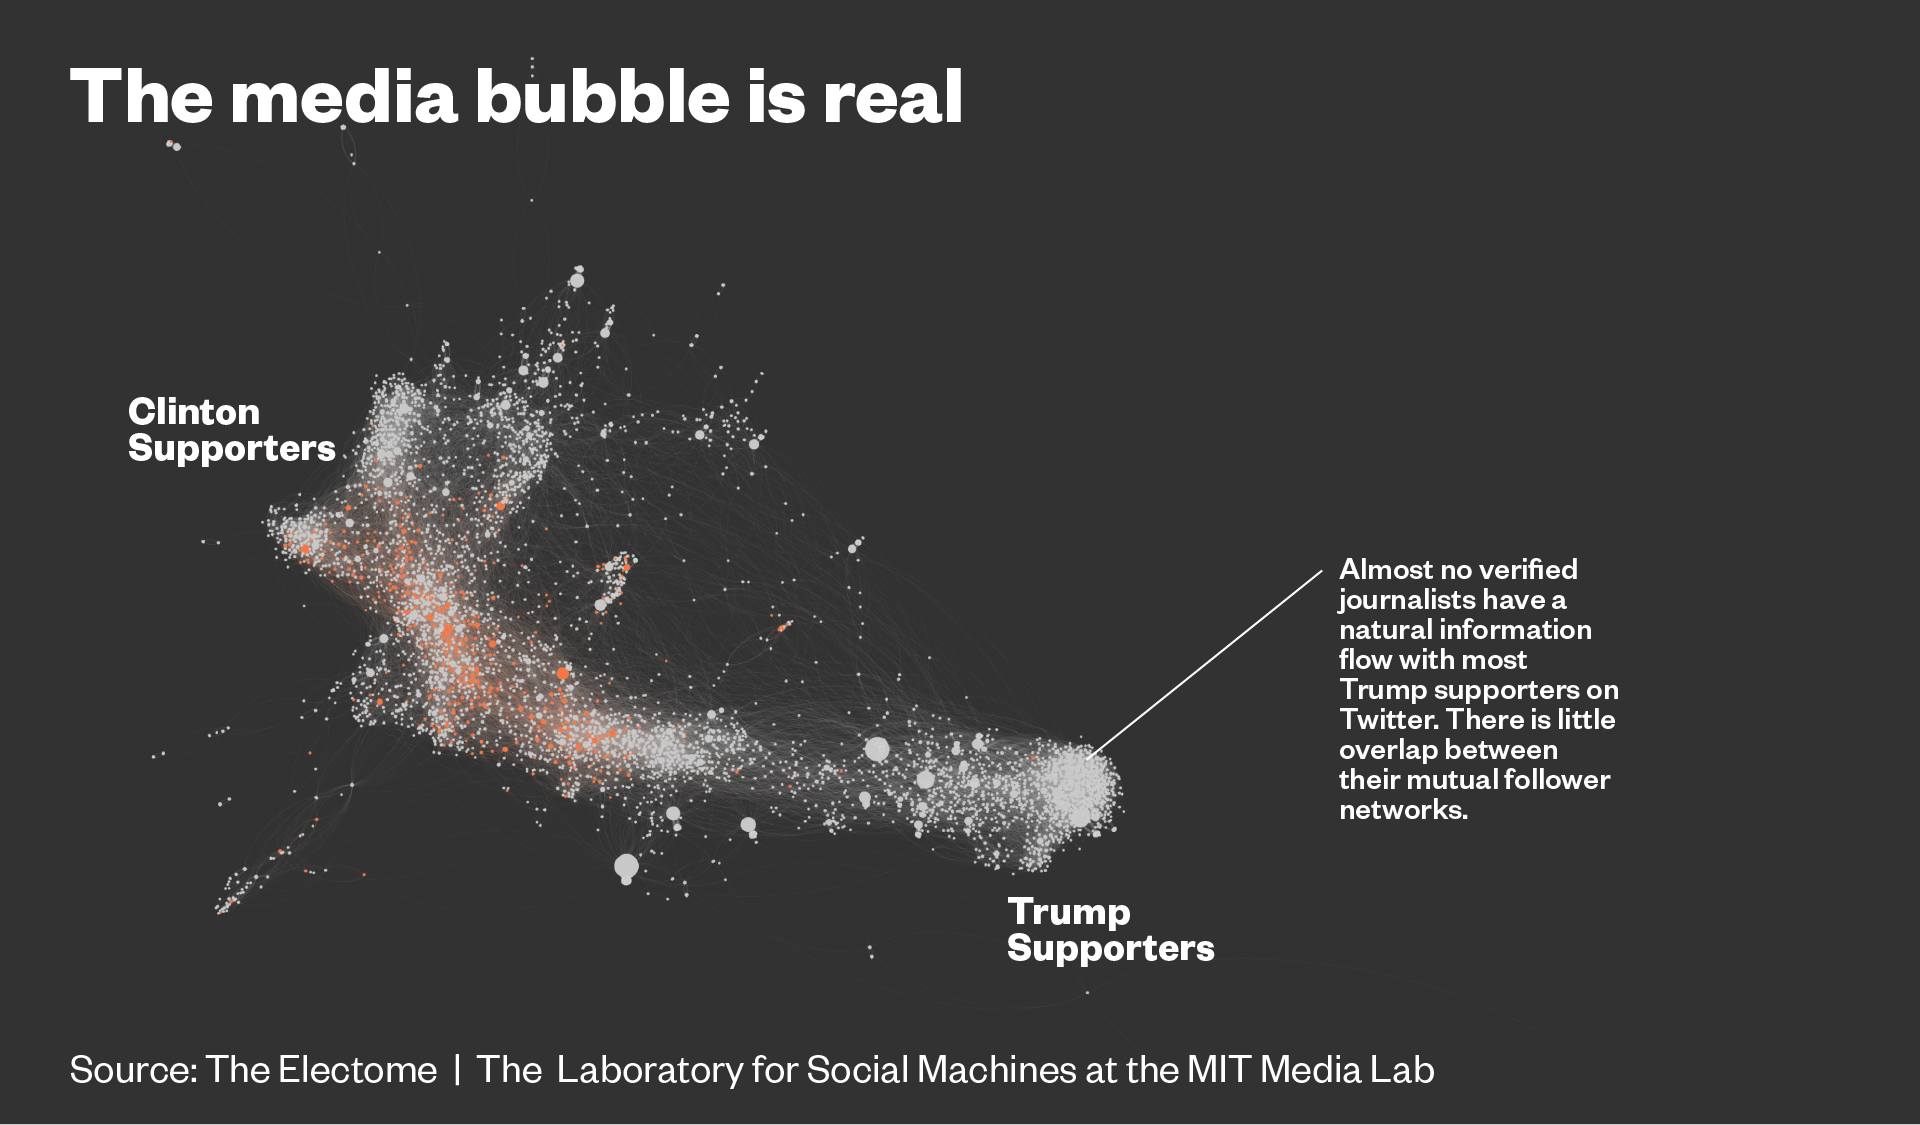
\includegraphics[width=\linewidth]{./images/election.png}
    \caption{Twitter follow networks for key influencers in the 2016 U.S. Presidential Election}
    \label{election}
\end{figure}

\section{Assessing Cluster Quality}
There are several methods for evaluating the quality of clusters. Leskovec et al. at Stanford performed an emperical comparision of several community detection algorithms, including the spectral-based graph partitioning method Local Spectral (similar to Spectral Bisection below), and the flow-based partitioning algorithm Metis+MQI (similar to Edge Betweenness below) \cite{Leskovec:2010:ECA:1772690.1772755}. They apply these methods to various data sets.
\par
The primary community score metric they use is conductance. Conductance measures cluster quality by looking at the ratio of edges in the community to the number of edges that leave that community. Formally, conductance is expressed as:

\begin{align}
    \phi(S) &= \frac{c_S}{min(Vol(S), Vol(V \setminus S))} \\
    c_S &= |{(u, v) : u \in S, v \notin S}| \\
    Vol(S) &= \sum_{u \in S}d(u)
\end{align}

where $S$ is the set of nodes in the community, $d(u)$ is the degree of node $u$. This captures both the connectedness of the community, as well as the connectedness of the community to the rest of the graph. The obejctive for a community detection algorithm is to minimize conductance.
\par
The authors identify that there are two key criteria for assessing the quality of clusters, the number of edges within a cluster, and the number of edges that join that cluster with the rest of the graph. They group the remaining quality scores into two groups, those that depend on both of these criteria (multi-criterion scores), and those that depend on only one of these criteria (single criterion scores) \cite{Leskovec:2010:ECA:1772690.1772755}.
\par
It is evident that conductance is a multi-criterion score as is depends on edges within the community as well as edges that leave the community. There are several other multi-criterion scores including expansion, internal density, and cut ratio. Expansion is given as:

\begin{align}
    f(S) &= \frac{c_S}{n_S}
\end{align}

where $c_S$ is the number of edges on the boundary of set $S$, and $n_S$ is the number of nodes in $S$. Internal density is given as:

\begin{align}
    f(S) &= 1 - \frac{m_S}{n_S(n_S - 1)/2}
\end{align}

where $m_S$ is the number of edges in $S$. Finally, cut ratio is given as:

\begin{align}
    f(S) &= \frac{c_S}{n_S(n - n_S)}
\end{align}

where $n$ is the number of nodes in the entire graph. One key single cirterion score is modularity, which is given by:

\begin{align}
    f(S) &= \frac{1}{4m}(m_S - E(m_S))
\end{align}

where $E(m_S)$ is the expected number of edges in a random graph where the degrees of each node remain the same as the original community $S$. This measure is discussed more under Modularity.

\section{Algorithms}
Several algorithms have been introduced to mine communities from connection information. Several of these algorithms are discussed here, along with details of my reimplementation of these algorithms.

    \subsection{Spectral Bisection}
    The spectral bisection method for detecting communities in graphs proposed by Pothen et al. involves using the eigenvectors of the Laplacian matrix for a graph to determine where to cut the graph \cite{doi:10.1137/0611030}. The Laplacian matrix for a graph is given by:

    \begin{align}
        L &= D - A
    \end{align}

    where $D$ is the diagonal matrix containing the degrees of each vertex, and A is the adjacency matrix for the graph. Once this matrix is found, the graph can be divided by taking the median value $x$ of the eigenvector with the second lowest eigenvalue of the Laplacian matrix. The graph is then split into two sets, $A$ and $B$ where $A$ has verticies whose components are less than or equal to $x$, and $B$ has all vertices whose components are greater than $x$. If the difference in the sizes of these sets is greater than one, verticies whose components equal $x$ are arbitrarily reassigned to $B$ until the difference in the sizes of $A$ and $B$ is one.
    \par
    We then consider the set of edges who have one vertex in $A$ and another vertex in $B$. This is an edge separator of the graph, taken from the bipartite graph contained in $A$ and $B$. With this edge separator, it is possible to compute the minimum vertex cover of the bipartite graph contained in $A$ and $B$. This cover is then used as the vertex separator to divide the graph into two parts.
    \par
    This method works well when the graph is easily separable into two distinct groups, however, it struggles when the graph is not easily separable \cite{Newman2004}.

    \subsection{Edge Betweenness}
    In 2002, Girvan and Newman developed a new partitioning method by looking at the edges that are least central to communities. This development was motivated by shortcomings of a heirarchical clustering algorithm when applied to community detection. The issue Girvan and Newman found was that the heirarchical method would often take a vertex that shared a single edge with a community, and split this vertex into a community of its own. Girvan and Newman thought it was intuitive that a vertex that has only one edge should belong to the community that contains the vertex at the other end of that edge \cite{Girvan7821}.
    \par
    To account for this, Girvan and Newman developed a new method for partitioning a graph based on looking for edges that are the most "between" communities, rather than looking at those that are most central to the communities as heirarchical clustering does. Instead of iteratively adding the strongest edges to a set of verticies, the new method iteratively removes edges from the original graph. Girvan and Newman extend Freeman's betweenness centrality to determine the edges that are the most between communities.
    \par
    Freeman's betweenness centrality is based off of finding the shortest path connecting two nodes. More formally, the betweenness centrality for some vertex $k$ is the number of shortest paths between all other pairs of verticies $i$ and $j$ such that the shortest path between $i$ and $j$ contains $k$. Girvan and Newman generalize this to apply to edges, where the betweenness of an edge is defined as the number of shortest paths that run along that edge.
    \par
    Once the betweenness has been calculated for all edges in the graph, the edge with the highest betweenness is removed. The betweenness is then recalculated for the new graph, and the next edge with the highest betweenness is removed. This process repeats until there are no more edges in the graph.

    \subsection{Modularity}
    Using modularity to detect communities in graphs was first proposed by Newman in 2006 \cite{Newman2006}. Newman identified that many community mining methods assume the network divides appropriately into subgroups, however, real-world social networks rarely behave this way. Instead, users can belong to several communities. In addition, typical graph partitioning algorithms are not suited well for community detection. These methods usually use minimum cut to divide the graph into subgroups. This is an intuitive method to apply, as it will minimize the number of edges running between the communities. However, you may need to constrain the size of the communities to prevent trivial solutions to dividing the network. For example, if the goal is to minimize edges between groups, the most straight-forward solution would be to create two groups, one of which is empty and one of which contains the rest of the network. This produces a count of edges between groups of zero. This trivial solution can be avoided by saying there needs to be at least $k$ nodes in each subgroup, but this requires determining this value ahead of time. Because of this, Newman was motivated to develop a new community detection method that is more applicable to real data.
    \par
    One goal Newman had was to eliminate the dependency on constraining the subgroup sizes as is required by typical graph partitioning algorithms. This would avoid the problem of trivially dividing a network into two subgroups where one is empty and the other contains the rest of the graph. To achieve this, Newman introduces the modularity matrix. The modularity matrix is defined using the following equation for each element of the matrix \cite{Newman2006}:

    \begin{align}
        B_{ij} &= A_{ij} - E_{ij} \\
        E_{ij} &= \frac{k_ik_j}{2m}
    \end{align}

    Where $A_{ij}$ is the count of the edges between nodes $i$ and $j$, and $E_{ij}$ is the expected number of edges between the two nodes, given that $k_n$ is the degree of some node $n$ and $m$ is the total number of edges in the network. One important property of this matrix is that all of the rows and columns sum to zero, meaning it has an eigenvector (1, 1, 1,...) with an eigenvalue of zero. This is similar to the Laplacian Matrix from the Spectral Bisection Method. This matrix is then represented as a linear combination of normalized eigenvectors.
    \par
    The method for dividing the network into groups is borrowed from Spectral Partitioning. Newman repeatedly selects the largest, positive eigenvalue as the basis for dividing the network. The network is then divided based on the values in the eigenvector, where positive values are grouped together and negative values are grouped together. It can also be noted that the magnitude of these values indicate the strength of which an element belongs to a subgroup. Large values indicate an element belongs with a group, while values close to zero indicate the element may fall between the two groups.
    \par
    This process continues until there are no more positive eigenvalues for the modularity matrix. This allows the algorithm to stop once the network is indivisible, while also preventing the need for determining the size of the subgroups ahead of time.

    \subsection{Walktrap}
    In 2005, Pascal Pons and Matthieu Latapy introduced an entirely different method for finding community structure in networks. Their method, named Walktrap, is based on repeated random walks through the graph. The method is motivated by the intuition that a random walk through a densely connected region of the graph will tend to stay within that region \cite{10.1007/11569596_31}.
    \par
    This algorithm makes several assumptions about the data, including that the graph is connected, and that there is an edge between every node and itself. The algorithm begins by dividing the entire graph of $n$ verticies into $n$ communities of one node each. These communities are then iteratively merged based on a distance measure $r$. The authors define the distance between two communities, $r_{ij}$, based on the probability of encountering node $j$ given a random walk from $i$ of length $t$, $P^t_{ij}$. It is important to note that for a sufficiently high value of $t$, the probability of ariving at node $j$ approaches $\frac{k_j}{2m}$ where $k_j$ is the degree of node $j$ and $m$ is the number of edges in the graph. In other words, the probability of arriving at a node depends only on the degree of that node, and not the starting node for the random walk. The authors formally define distance by the equation:

    \begin{align}
        r_{ij} &= \sqrt{\sum^n_{k=1}{\frac{(P^t_{ik} - P^t_{jk})^2}{d(k)}}}
    \end{align}

    This measure compares the probability of arriving at the same node $k$ when starting from both nodes $i$ and $j$. If the probabilities of arriving at $k$ are similar for all nodes in the graph, then the distance between $i$ and $j$ is small and they are likely part of the same community. Conversely, if the probabilities of arriving at $k$ differ for many entries in the probability lists, $i$ and $j$ are likely not in the same community.
    \par
    The authors note that their algorithm works well for short random walks fo $3 <= t <= 8$. The authors also advise decreasing $t$ if the graph is dense, and increasing $t$ if the graph is sparse. This is because the convergence speed of a random walk increases as the density of the graph increases \cite{10.1007/11569596_31}.

\section{Evaluation}
To examine the usefulness of these algorithms, I will use them to detect communities in Stack Overflow data. I will compare the performance of my implementations against existing implementations in the igraph package. This will provide insight into the correctness of my implementations as the results should be very similar when compared against igraph. The Stack Overflow data is contains a table of questions, a table of answers to those questions, and a list of tags associated with each question. In the questions and answers tables, there are also fields indicating the user who posted the question. In this data, community structure exists in the form of questions that are about related topics. For example, we would expect a user who is active in the C++ community to answer many questions about C++. It is also possible for users to be active in multiple different communities.
\par
Initially I thought it would be useful to represent both users and questions in the graph we are mining for communities, however, this proved to not be useful. Representing both users and questions forms a bipartite graph where all edges go between user and question nodes. Although this better represents the original data, this makes it much harder to do community detection. For example, if a user is active in multiple communities, there will be more connections joining these communities and it will be harder to find the community structure.
\par
To account for this, I manipulated the graph to better encode the tag information. To do this I removed the user nodes, and created edges between questions that share a tag. It can be seen that this will significantly increase the connectedness of the graph, but this connectedness is useful for algorithms such as Walktrap.

% TODO: implement and evaluate methods

\section{Conclusion}

\newpage
\bibliography{sources}
\bibliographystyle{plain}

\end{document}
